In this course, we start with considering a smooth embedding of a surface
in \(\mathbb{R}^3\) as we call it to be a regular surface.
\begin{enumerate}[(1)]
    \item \(M\) has the Riemannian metric induced by the Euclidean metric
    of \(\mathbb{R}^3\). This is equivalent to saying \(M\) with this induced
    metric is isometrically embedded in \(\mathbb{R}^3\).
    \item The \engordnumber{2} fundamental form tells us how \(M\) looks
    like in \(\mathbb{R}^3\).
\end{enumerate}

Later, we studied the Gauss's elegant theorem, which says the Gaussian
curvature is determined by the Riemannian metric (\engordnumber{1}
fundamental form) only. Since the curvature is a local property,
by choosing a suitable local coordinate, we have the following convenient
expression of the Gaussian curvature. 
\begin{enumerate}[(1)]
    \item In geodesic polar coordinate \((r,\theta)\)
    \[
        ds^2=dr^2+G(r,\theta)d\theta^2    
    \]
    \[
        \Rightarrow K=-\frac{(\sqrt{G})_{rr}}{\sqrt{G}}    
    \]
    \item By a profound fact that a regular surface is locally conformally
    flat, there always exists isothermal coordinates on \(S\), such that 
    \[
        ds^2=\lambda((dx^1)^2+(dx^2)^2)\quad \lambda>0 \text{ is smooth on }
        S    
    \]
    \[
      K=-\frac{1}{2}\Delta_{ds^2}\log \lambda=
      -\frac{1}{2\lambda}  \Delta_{\mathbb{R}^2}\log \lambda
    \]
    \item If \(p\in S\) is not umbilical, then near \(p\) we can use 
    the curvature lines as coordinate lines. In this case,
    \[
        ds^2=g_{11}(dx^1)^2+g_{22}(dx^2)^2    
    \]
    \[
        II=h_{11}(dx^1)^2+h_{22}(dx^2)^2    
    \]
    \[
        K=-\frac{1}{\sqrt{g_{11}g_{22}}}
        \left(
            \partial_1\left(
                \frac{\partial_1 \sqrt{g_{22}}}{\sqrt{g_{11}}}
        \right)
        +
            \partial_2\left(
                \frac{\partial_2 \sqrt{g_{11}}}{\sqrt{g_{22}}}
        \right) 
        \right) 
    \]
\end{enumerate}
No matter in which expression as above, we see the Gaussian curvature is
of ``the \engordnumber{2} order derivative of the metric''. In particular,
in the first two expressions, \(K\) is a \engordnumber{2} order derivative
of some function that determines the metric. Now we can ask the following
questions
\begin{enumerate}[\underline{Question} 1]
    \item (Prescribed Gaussian curvature problem) 
    
    Given any smooth function
    \(K=K(x,y)\) on \(S\), can we determine the metric?

    (As we can guess from above, this problem is equivalent to the 
    solvability of a \engordnumber{2} order PDE problem. To further
    explore this question, we can first divide the manifolds into 
    two categories: closed (compact without boundary), or complete 
    non-compact manifolds. On a cloesed surface, the Gauss-Bonnet gives 
    certain restriction on \(K\). One can further look at Kazdan-Warner's
    paper in 1974(Annals) for detailed discussions)
    \item Given a 2-dimensional Riemannian manifold \((S,g)\), can we
    isometrically embed or immerse it into \(mathbb{R}^3\), \ie\ can such
    \(g\) come from the Euclidean metric in \(\mathbb{R}^3\)?
    If so, how smooth of such embedding or immersions map could be?

    (Hilbert's theorem has told us we can not isometrically immerse 
    a hyperbolic plane into \(\mathbb{R}^3\). If a surface in \(\mathbb{R}^3\)
    is closed \(S\) must have an elliptic point. Hence, 
    we can easily exclude the closed case, \ie\ a closed surface with \(K=-1\)
    can never embedded or immersed into \(\mathbb{R}^3\) smoothly. 
    (indeed as an affirmative answer of question 1 above, there always exists
    a metric with \(K=-1\) on a closed surface with genus \(g\ge 2\). 
    Moreover, the universal covering of such surface is just the hyperbolic
    plane.)
    However, if we relax the smooth embedding/immersion, the Nash-Kuiper's 
    theorem says we can isometrically embed or immerse hyperbolic plane
    or higher genus torus into \(\mathbb{R}^3\) in a \(C^1\)-way. Intuitively,
    these surfaces in \(\mathbb{R}^3\) look like corrugated surfaces.
    )
    As another remark on a torus (\(g=1\)), there always exists a metric
    with \(K=0\), such torus is usually called to be a flat torus. This flat
    torus is not isometrically embedded or immersed into \(\mathbb{R}^3\) in
    a smooth way.
    \begin{center}
        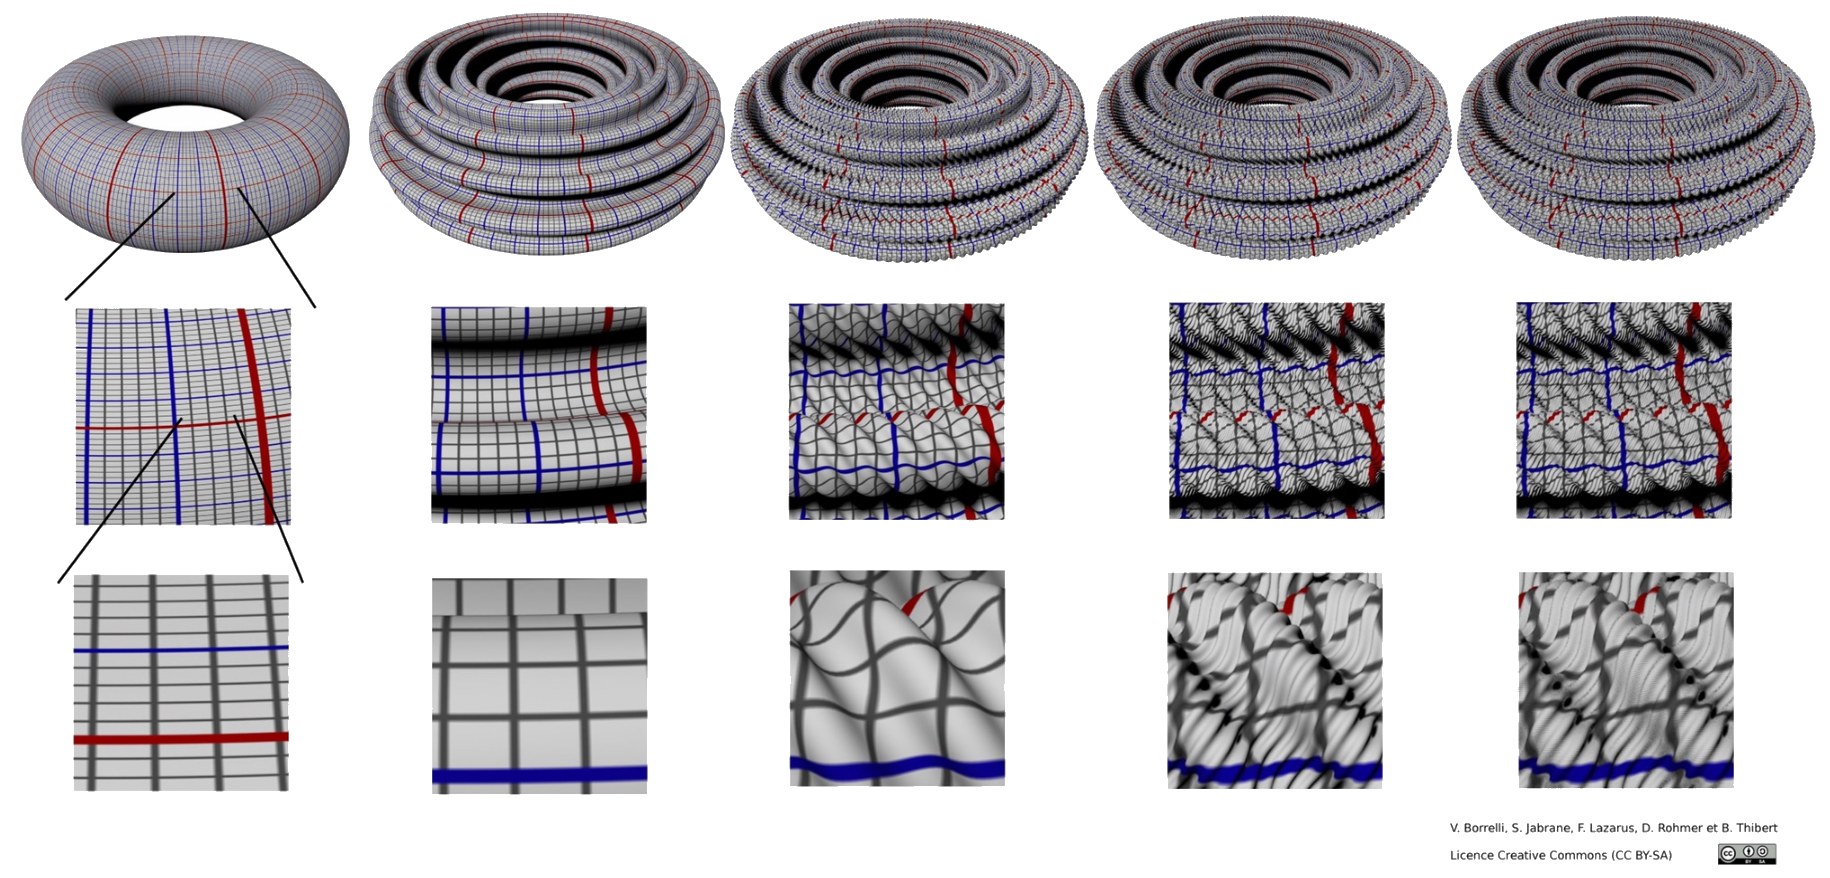
\includegraphics[scale=0.3]{picture/final remark/corrugated.png}
    \end{center}
    This shows how to isometrically embed a flat torus into \(\mathbb{R}^3\)
    in a \(C^1\)-manner.
    \begin{theorem}[Nash Embedding theorem]
        \((M^m,g)\) is a smooth Riemannian manifold, then \(M\) can 
        be smoothly isometrically embedded into \(\mathbb{R}^{
            \frac{(3m+11)m}{2}
        }\)
        \begin{enumerate}[(1)]
            \item if \(M\) is compact, then 
            \(M\hookrightarrow \mathbb{R}^n\) with 
            \(n\le m(m+1)\)
            \item if \(M\) is non-compact, then \(M 
            \hookrightarrow \mathbb{R}^n\) with 
            \(n\le \frac{3m+11}{2}\)
        \end{enumerate}
    \end{theorem}
    \underline{Recall}: you might have seen from another course
    that 
    \begin{theorem}[Whithey's embedding theorem]
        \(M^m\) is a smooth manifold, then \(M^m\) can be smoothly embedded in
        \(\mathbb{R}^{2m}\).
    \end{theorem}
\end{enumerate}
\vspace{4cm}
\begin{center}
    {\Huge To Be Continued...}    
\end{center}
